\documentclass[12pt, letterpaper] {article}

\parindent=5mm
\usepackage[spanish]{babel}

\usepackage{amssymb}
\usepackage{amsmath} 
\usepackage{amsfonts}

\usepackage[numbers,sort&compress]{natbib}
\usepackage{graphicx}

\usepackage{url}
\usepackage{hyperref}

\usepackage[top=25mm, bottom=20mm, left=1.5cm, right=1.5cm]{geometry}
\setlength{\parskip}{2mm}
\setlength{\parindent}{1pt}

\usepackage{listings}

\usepackage{float}

\usepackage[utf8]{inputenc}
\usepackage{graphicx} 
\usepackage{subfigure} 

\usepackage{color}
\usepackage{multirow}

\definecolor{dkgreen}{rgb}{0,0.6,0}
\definecolor{gray}{rgb}{0.5,0.5,0.5}
\definecolor{mauve}{rgb}{0.58,0,0.82}

\usepackage{color}
\usepackage{listings}
\lstset{ %
  language=R,                     % the language of the code
  basicstyle=\footnotesize,       % the size of the fonts that are used for the code
  numbers=left,                   % where to put the line-numbers
  numberstyle=\tiny\color{gray},  % the style that is used for the line-numbers
  stepnumber=1,                   % the step between two line-numbers. If it's 1, each line
                                  % will be numbered
  numbersep=5pt,                  % how far the line-numbers are from the code
  backgroundcolor=\color{white},  % choose the background color. You must add \usepackage{color}
  showspaces=false,               % show spaces adding particular underscores
  showstringspaces=false,         % underline spaces within strings
  showtabs=false,                 % show tabs within strings adding particular underscores
  frame=single,                   % adds a frame around the code
  rulecolor=\color{black},        % if not set, the frame-color may be changed on line-breaks within not-black text (e.g. commens (green here))
  tabsize=2,                      % sets default tabsize to 2 spaces
  captionpos=b,                   % sets the caption-position to bottom
  breaklines=true,                % sets automatic line breaking
  breakatwhitespace=false,        % sets if automatic breaks should only happen at whitespace
  title=\lstname,                 % show the filename of files included with \lstinputlisting;
                                  % also try caption instead of title
  keywordstyle=\color{blue},      % keyword style
  commentstyle=\color{dkgreen},   % comment style
  stringstyle=\color{mauve},      % string literal style
  escapeinside={\%*}{*)},         % if you want to add a comment within your code
  morekeywords={*,...}            % if you want to add more keywords to the set
} 

\usepackage{booktabs}
\usepackage[table,xcdraw]{xcolor}


\author{Ricardo Rosas Macías}

\title{Práctica 2. Autómata celular}

\date{\today}

\begin{document}

\maketitle



\section{Introducción}

El experimento es un modelo matemático llamado autómata celular, este realiza una secuencia parecida a una máquina de Turing que puede ser representada matemáticamente con una matriz booleana para así obtener la interacción que esta tiene a  través del tiempo. 

 \section{Objetivo}
El interés en el trabajo presente es examinar la supervivencia celular, durante la evolución celular que tiene el experimento. Asimismo, observar cómo la probabilidad afecta en la supervivencia.

 \subsection{Descripción}

Se busca \cite{elisawebAC}:
\begin{quotation}
 ``Diseñar y ejecutar un experimento para determinar el número de iteraciones que procede la simulación en una malla de 30 por 30 celdas hasta que se mueran todas, variando la probabilidad inicial de celda viva entre cero y uno en pasos de 0.10.''
\end{quotation}

\section{Resultados y conclusiones}

Para realizar el código se  tomo lo anteriormente reportado \cite{MPP2}\cite{EP2}. En las líneas de código de la parte inferior se determinaron los parámetros con los que se ejecuta para variar la probabilidad de supervivencia.

\begin{lstlisting}[language=R]
dim <- 30
num <- dim^2
limit <- 10
repeatexp <- 30
probability <- seq(from=0.1, to=0.9 ,by=0.10)

results <- data.frame()

for(p in probability){
  iterations <- list()
  actual <- matrix(1 * (runif(num) < p) , nrow=dim, ncol=dim)
  suppressMessages(library("sna"))
  for (rep in 1:repeatexp){
    if(sum(actual) == 0){ 
      iterations <- c(iterations, 0)
      iterations <- unlist(iterations)
    } else if(sum(actual) == num){
      iterations <- c(iterations , 0)
      iterations <- unlist(iterations)
    } 

  iterations <- c(iterations, iteracion)
      iterations <- unlist(iterations)
    }
  }
   results <- rbind(results, iterations)
system("convert -delay 50 -size 300x300 p2_Rep1_t*.png -loop 0 AC.gif") 
\end{lstlisting}


Además, con la paquetería \textit{ggplot2} se obtuvo la visualización de código en la figura \ref{ProbI}, que muestra la distribución de los datos en donde se aprecia la densidad de probabilidad. Por consiguiente, la probabilidad 0.3, 0.4 y 0.5 tienen la misma expectativa de vida; de tal manera que no tienen limite de iteraciones y los agentes tienen menor auspicio a morir. Por otro lado, la probabilidad de 1 tiene la mayor posibilidad de estar viva, ya que esta tiene menor iteraciones con los vecinos.

\begin{figure}[H]
\centering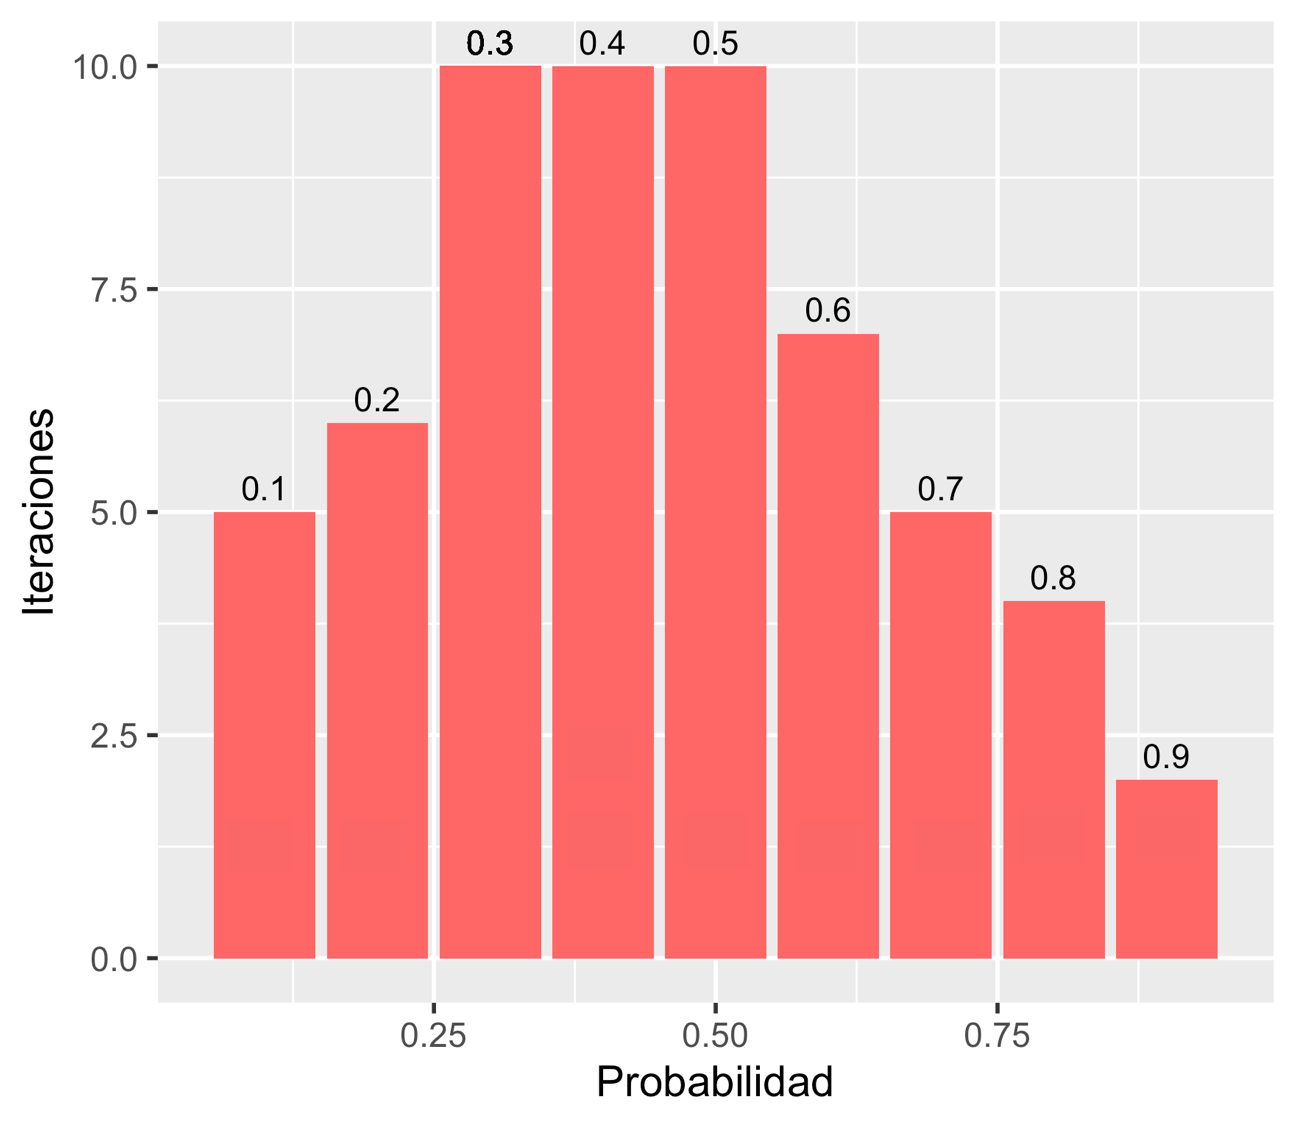
\includegraphics[width=92mm]{Probainter.png}
\caption{Probabilidad respecto a la iteración}
\label{ProbI}
\end{figure}

Para observar el fenómeno descrito anteriormente, se creó un gif de las imágenes proporcionadas del experimento; en las líneas de la parte inferior del código, de modo que en la figura \ref{AutC} se puede ver el inicio de los agentes en la matriz y la evolución rápida de los agentes respecto a sus vecinos. 

\begin{figure}[H]
\centering
\subfigure[inicio]{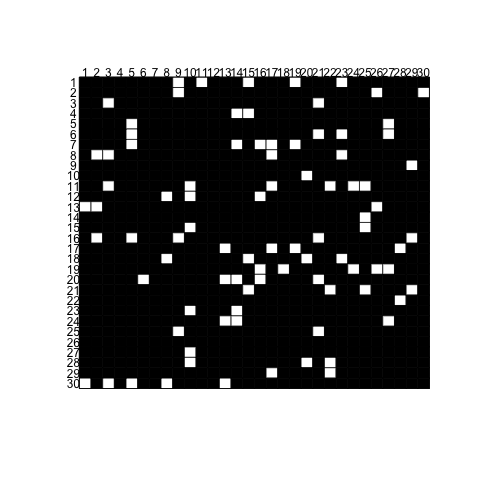
\includegraphics[width=68mm]{./p2_Rep1_t0}}\vspace{-1mm}
\subfigure[Paso 1]{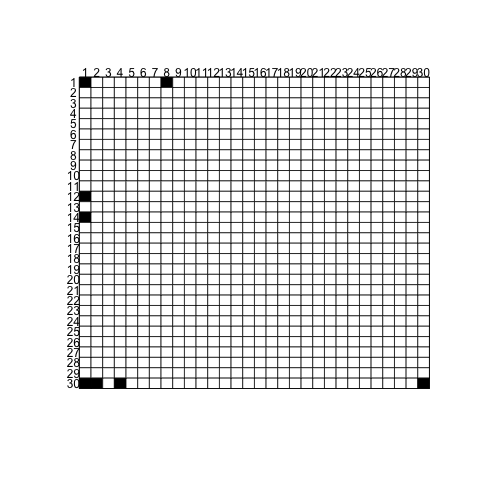
\includegraphics[width=68mm]{./p2_Rep1_t1}}\vspace{-1mm}
\subfigure[Paso 2]{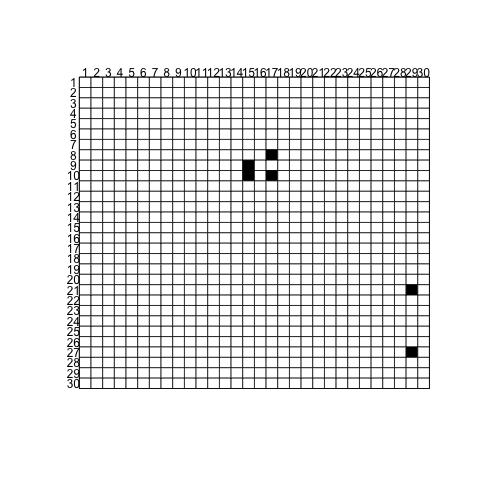
\includegraphics[width=68mm]{./p2_Rep1_t2}}\vspace{-1mm}
\subfigure[Paso 3]{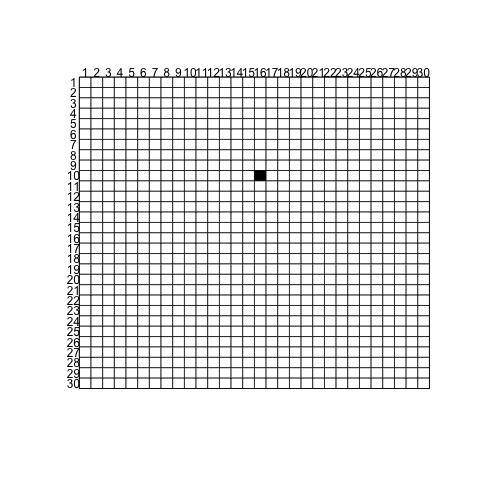
\includegraphics[width=68mm]{./p2_Rep1_t3}}
\caption{Matriz de evolución de agentes}\label{AutC}
\end{figure}

\bibliographystyle{plainnat}

\bibliography{BHWP2}


\end{document} 